\chapter{The Principles} \label{CHAP:PRINCIPLES}

\section{The fifteen principles}

The 15 principles are demonstrated on the ternary CAM \textbf{(content-addressable memory)} problem:

Overview:

\begin{tabular}{|c|c|c|}
\hline 
\textbf{Number} & \textbf{Principle} & \textbf{Used in} \\ 
\hline 
P1 & Avoid obvious waste & Zero-copy interfaces \\ 
\hline 
P2 & Shift computation in time &  \\ 
P2a & Precompute & Application device channels \\ 
P2b & Evaluate lazily & Copy-on-write \\ 
P2c & Share expenses, batch & Integrated layer processing \\ 
\hline 
P3 & Relax requirements &  \\ 
P3a & Trade certainty for time & Stochastic fair queuing \\ 
P3b & Trade accuracy for time & Switch load balancing \\ 
P3c & Shift computation in space & IPv6 fragmentation \\ 
\hline 
P4 & Leverage off system components &  \\ 
P4a & Exploit locality & Locality-driven receiver \\
P4b & Trade memory for speed & Processing; Lulea IP lookups \\
P4c & Exploit existing hardware & Fast TCP checksum \\
\hline 
P5 & Add hardware &  \\ 
P5a & Use memory interleaving and pipelining & Pipelined IP lookups \\ 
P5b & Use wide word parallelism & Shared memory switches \\ 
P5c & Combine DRAM and SRAM effectively & Maintaining counters \\ 
\hline 
 &  & \textbf{Networking examples} \\ 
\hline 
P6 & Create efficient specialized routines & UDP Checksums \\ 
\hline 
P7 & Avoid unnecessary generality & Fbufs \\ 
\hline 
P8 & Don't be tied to reference implementation & Upcalls \\ 
\hline 
P9 & Pass hints in layer interfaces & Packet filters \\ 
\hline 
P10 & Pass hints in protocol headers & Tag switching \\ 
\hline 
P11 & Optimize the expected case & Header prediction \\ 
P11a & Use caches & Fbufs \\ 
\hline 
P12 & Add state for speed & Active VC list \\ 
P12a & Compute incrementally & Recomputing CRCs \\ 
\hline 
P13 & Opt. degrees of freedom & IP trie lookups \\ 
\hline 
P14 & Use bucket sorting, bitmaps & Timing wheels \\ 
\hline 
P15 & Create efficient data structures & Level-4 switching \\ 
\hline 
\end{tabular} 

Categorization: The principles can be divided into different subcategories,

Principles 1 to 5 are called \textbf{system principles}, 6 to 10 \textbf{Improving efficiency while retaining modularity} and 11 to 15 \textbf{speeding it up}.  

Examples for each principle:

\textbf{P1}: Look for obvious waste in the computation of similar expressions and only calculate them once. For instance $i = 5.1 * n + 2$ is calculated and later $j = (5.1 * n+ 2) *4$, which can obviously use the first result.

\textbf{P2}: Systems have aspect in space time, \textbf{space} refers to geographic distribution of subsystems, \textbf{time} refers to the fact that a system is instantiated at different time scales (fabrication time, compile time, parameter setting time, run time), shifting computation in time can lead to more efficiency.

\textbf{a)} Precompute: For instance, you have a DSP which needs to generate a sinusoidal signal. The samples of the sinusoidal can be precomputed and stored in a table.

\textbf{b)} Evalute lazily: Example is \textbf{copy on write}, only copy data when you want to perform a write operation, not before.

\textbf{c)} Share expenses: For instance \textbf{batching}, multiple expensive operations are computed together, which may be more efficient than doing them one after another.

\textbf{P3}: Relax System Requirements: Typical layered systems designed in a top-down approach divide functionalities on subsystems on different layers. This is good for abstraction but may have negative effects on efficiency.

\textbf{a)} Trade Certainty for Time: Make use of probabilities. An example is Cisco's netflow, when there is no capacity to count packets, it will count random samples and statistically extrapolate those and the count will be correct to a certain precision.

\textbf{b)} Trade Accuracy for Time: To gain efficiency you can reduce accuracy of operations in some cases. Multimedia processing often relies on lossy compressions which accuracy may be reduced to gain performance. (For instance replace divide by shift and lose a little accuracy)

\textbf{c)} Shift Computation in Space: Some subsystems may have to adapt to loose requirements introduced in other subsystems, which is called \textbf{shifting computation in space}. Example, routers need to fragment packets is avoided by having end systems calculate packet sizes that will pass all routers.

\textbf{P4}: Leverage of System components, top-down provides good modularity, partial bottom-up design may be required for performance critical applications.

\textbf{a)} Exploit locality: Memory hardware offers efficiencies if data is laid out contiguously, same sector for disks or same DRAM page for DRAM, disk-search algorithms exploit this and IP-lookup algorithms reduce lookup times by placing several keys in a wide word.

\textbf{b)} Trade memory for speed: Lulea IP-lookup uses sparse arrays that can be looked up efficiently by space-efficient bitmaps.

\textbf{c)} Exploit hardware features: \textit{Strength reduction} is used to optimize away multiplications in loops (compilers do this).

\textbf{P5}: Add hardware to improve performance, if nothing works buy new hardware, faster processor, faster and more memory and so on which may even be more cost effective than trying to solve every problem.

\textbf{a)} Use Memory Interleaving and Pipelining: From Chapter 2, Micro-opt., similar techniques are used in IP-lookups, classification and scheduling algos. 

\textbf{b)} Use wide word parallelism: Common technique in many networking designs, example is \textit{Lucent bit vector scheme}, use wide memory words that can be processed in parallel.

\textbf{c)} Combine DRAM and SRAM: SRAM expensive and fast, DRAM cheap and slow, combination of the two to get best benefit. SRAM as a cache, DRAM as database is classical. But SRAM can be used for efficient key lookups and so on, whereas the data itself lies on DRAM.

\textbf{P6}: Efficient specialized routines, specialized routines can be more efficient for specific purposes than general-purpose routines.

\textbf{P7}: Avoid unnecessary generality, remove features to gain performance (features that are almost never used). 

\textbf{P8}: Don't be tied to reference impl., reference implementations are often overspecified and also designed to clearly state what has to be done and not for efficiency.

\textbf{P9}: Pass hints in module interfaces, pass information that lets a service avoid unnecessary computation, cache lookups and so on.

\textbf{P10}: Pass hints in protocol headers, circumvent inefficiencies in message-passing parallel systems by passing hints in message headers (carry address of interrupt handler for fast dispatch of an operation).

\textbf{P11}: Optimize the expected case, should be rather obvious, heuristically determine which case appears most often and optimize it. Handle infrequent cases that require more difficult logic.

\textbf{a)} use caches: Keep data required for the computation of expected cases in cache. When an infrequent case appears where data is not in the cache, it will have to be looked up, however it should be statistically improbable.

\textbf{P12}: Add or exploit state to gain speed, add redundant information to expensive operations to speed up the process. Classical example is the use of secondary indices in databases.

\textbf{a)} Compute incrementally: Example, incremental comp. of IP checksums when only few fields change.

\textbf{P13}: Optimize degrees of freedom, using special datastructures or algorithms some degrees of freedom may be overlooked. For example, multibit trie IP lookup algorithms overlook the DoF, that the number of bits used to index a trie node can vary.

\textbf{P14}: Special techniques for finite universes such as integers, bucket sort, array looups and bitmaps may be more efficient than general purpose algorithms (for integers).

\textbf{P15}: Algorithmic techniques to create efficient data structures, in general P1 to P14 should be applied before thinking of special algorithmic techniques. But the author states that it is still worth while.

\subsection{Eight Cautionary Questions}
Questions you should ask yourself while impl. these principles for a given problem:

\begin{enumerate}
	\item Is it worth improving performance? It may not even be necessary..
	\item Is this really a bottleneck?
	\item What is the impact of this change on the rest of the system?
	\item Does initial analysis indicate significant improvement?
	\item Is it worth adding custom hardware?
	\item Can protocol changes be avoided?
	\item Do prototypes confirm the initial promise?
	\item Will performance gains be lost if the environment changes?
\end{enumerate}

\section{Principles in Action}

Concentrating on examples used in the slides here, since there are many more in the book..

\subsection{Ternary CAM}

Ternary content-addressable memory is used to speed up specific problems. For instance, router use a longest prefix match to find IP addresses of 32 bit length an hold 300.000 entries in their table. The question is, how to efficiently store and retrieve entries based on longest prefix match?

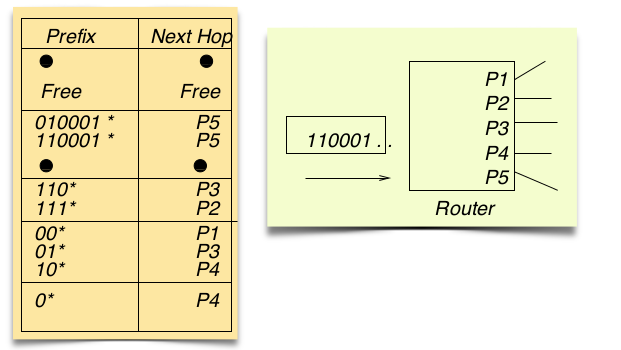
\includegraphics[width=.7\textwidth]{images/chap4/Ternary_CAM.png}

\textbf{Updating the table:} 

Ordering is done within prefixes of different length only. I.e. any \texttt{x.x.x.x/y} for constant \texttt{y} comes before \texttt{x.x.x.x/z} for $z > y$, but is not order for same addresses with prefix for \texttt{y}.

Free space is available at the beginning of the table. When an entry is inserted, holes are created by iteratively moving entries up. Starting at the top, a hole is created using the last element of prefix $i$, then proceed putting up elements for $i+k$, $i+k < 32$ and stop when a hole is available for the desired prefix length. Visually it looks as in the slides:

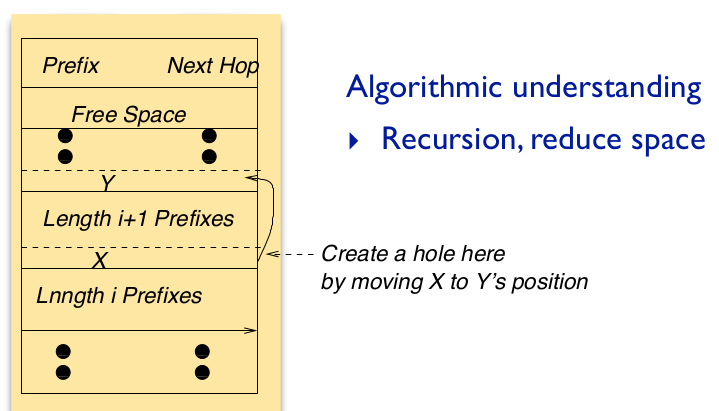
\includegraphics[width=.7\textwidth]{images/chap4/Ternary_CAM_update}

\subsection{Routing}

The Problem is, that a router wants to compute a lowest-cost path to a certain destination. In a more complex scenario, edges in the network are linked with different costs. Static routing protocols precompute paths for a router based on these link-costs and minimize path costs. Such static routing protocols are referred to as "link-state routing protocol" and routers send so called "link state packets" (LSP) that list their neighbors to all other routers.

When a router has all other LSPs, the network mapping is complete and \textbf{lowest-cost paths can be computed}, for example using \textbf{DJIKSTRA}s shortest path algorithm.

Priority queues for the link-costs are often used. However, general-purpose prio. queues such as heaps have at best a cost of $O(log N)$, leading to a complexity of $O(N log N)$ for the algorithm. Which fact can be exploited to speed up the process?

\textbf{Solution:} Since we have costs represented by small integers less than a natural number $k$ and a limited diameter (for instance, there will be no routes greater $15$ hops..), bucket sorting based priority queue can be used leading to amortized costs of $O(N + d \cdot m)$, $d = diameter, m = max \ cost$.

\subsection{LSP Fragmentation}

This was an actual problem that arose in the design of OSI and OSPF. Since routers send LSPs to all neighbors and vice versa, a lot of traffic is generated just by synchronizing routers. Packets greater the biggest MTU of 1500 bytes (at least for ethernet) have to be fragmented by routers so they are of size maximal 1500 bytes. This fragmentation is slow and expensive.

In the slide example, we have only 500 edges of 8 bytes each which is already greater than 1500 bytes. 

\textbf{Solution:} Modify Router $R1$ to be multiple routers $R1a, R1b, R1c$ with separate SQN. The set of routers connected to $R1$ is divided into multiple LSPs for pseudo-routers $R1a, \dots$ so the LSP of a pseudo-router doesn't exceed the maximal MTU. Hence, we don't have fragmentation on the network level anymore, although we fragment the packets ourselves...

Note the principal in action is \textbf{SHIFT COMPUTATION IN SPACE}!

\subsection{Quality of Service: Multicast IntServ}

Some technologies such as cable have multiple receivers listening to one connection (multicast). In the example receivers may specify which packets to receive (src/dsp address, port, protocol and so on). Therefore filters may have to be applied to huge amounts of data.

Hence the problem is

\begin{itemize}
    \item Matching against a lot of filters
    \item Multiple destinations for packets
\end{itemize}

\textbf{Solution:} Solutions include adding a field that denotes a \textbf{Flow Label}, similar to virtual circuits used in ATM.

\subsection{Resource Hogs}

Problem: Don't send packets faster than a certain rate, i.e., \texttt{B/T} bits per second.

One timer is not enough to limit the datarate, since violations of the contract are still possible. Assume, timer periods 0,T,2T,... periods having length T. Now we can have bursts ar one point in T breaking contract on a finer granularity than we measure. Hence, we need multiple timers, which on the other hand are expensive.

\textbf{Solution:} Add a random gap between the policing intervals since they need not be fixed! This way, over time, violations of contract will be encountered with a certain (by design high) probability.

\subsection{Resource Hogs Part II}

Problem: Find the user with the highest consumption, needs identification, probably some kind of sorting data structure such as priority queues.

To identify such a flow with high consumption, a statistic has to be created over many packets. It may not be sufficient to look at a time period of 5ms as some user may have micro bursts that over time don't amount to a lot of traffic.

However, creating a statistic of billions of packets with potentially thousands of different flows is expensive when performed naively.

\textbf{Solution:} \textit{Exponential (Binomial) Bucketing} of course! Relax the requirement, s.t. the accuracy can be off by a factor of 2. Aggregate users that are within a factor of 2 into the same group.

A bit in a bitmap is set if a bucket is non-empty. The resource hog is then in the bucket with the rightmost bit set. (Counting is still a problem, but another problem that is not solved here).







































